% Created 2024-12-10 Tue 23:54
% Intended LaTeX compiler: pdflatex
\documentclass[11pt]{article}
\usepackage[utf8]{inputenc}
\usepackage[T1]{fontenc}
\usepackage{graphicx}
\usepackage{longtable}
\usepackage{wrapfig}
\usepackage{rotating}
\usepackage[normalem]{ulem}
\usepackage{amsmath}
\usepackage{amssymb}
\usepackage{capt-of}
\usepackage{hyperref}
\author{Akilan}
\date{\today}
\title{}
\hypersetup{
 pdfauthor={Akilan},
 pdftitle={},
 pdfkeywords={},
 pdfsubject={},
 pdfcreator={Emacs 29.1 (Org mode 9.6.6)}, 
 pdflang={English}}
\begin{document}

\tableofcontents

\section{P2PRC tracking home server}
\label{sec:org5106d20}
\subsection{Abstract}
\label{sec:org119e303}
This is a library on top of P2PRC to create easier abstractions
to setup servers on spare laptops at home and run applications
which can exhibit a monolithic behaviour (Ex: Self hosted
jitsi, Invidious). The motivation is to ensure users can
share self hosted infrastructure with friends and can design
a really simple replicatable instances of servers.

\subsection{Problems being addressed}
\label{sec:orgb2d89d0}
\begin{enumerate}
\item Remembering ports mapped and stateful restart. Rather than the OS remember
information of the processes. The P2P network should also track it and
propagate it to other nodes in the network. This is to ensure when a process
fails there is a formally representable reason which can appropriate corrective
actions.
\item Arbitrary instructions used to start a process and should be remembered to reproduce a
process if a node is down.
\end{enumerate}


\subsection{What are attempting to do}
\label{sec:org0f074f0}
The section below describes in detail the ideal strategy of addressing the problems stated
above.

\subsubsection{Building Abstraction}
\label{sec:orgaee85d9}
We are proposing to build a library of the Haskell bindings which do the following:
\begin{itemize}
\item Creating a P2PRC process and allowing users to modify it's behaviour in functional manner with for instance
immutable datatypes.
\item Allowing users to run this abstraction in a reproducible manner or constraining it to run on precise
sets of machines.
\item Should be able to represent the deployment strategy used (ex: Nix, Ansible etc\ldots{}). This keeps the
deployment agnostic and not vendor specific.
\item The intended idea of this is to only work with monolithic applications.
\end{itemize}

\subsubsection{Building it for only home server users}
\label{sec:orgffcf4bf}
\begin{itemize}
\item The use case is to ensure it's easier to setup a set of servers and shuffle P2PRC processes around
when needed. We intend to do this by ensuring a process is represented as type.
\item Targets initially with the assumption that there is only 1 reliable root node to relay traffic to the make the setup
easier. Future plans will create a DNS layer which can make root nodes and P2PRC processes reproducible.
\end{itemize}

\subsubsection{Lenient rules}
\label{sec:orgfdab7c9}
\begin{itemize}
\item This library is built for home users, therefore the library will be setup for P2PRC using the \href{https://github.com/Akilan1999/p2p-rendering-computation/pull/115}{unsafe mode} which will ensure that all public
keys will be added to the \href{https://www.ssh.com/academy/ssh/authorized-keys-file\#:\~:text=The\%20authorized\_keys\%20file\%20in\%20SSH,keys\%20and\%20needs\%20proper\%20management}{SSH auth list} of all nodes available in the network. While this is not secure it
comes with pre-assumption that all nodes joining the network are home servers and are needed to access each other
with limited rules (set by user permission from the OS side).
\item We assume that all P2PRC processes run on a bare-metal machine without any virtualisation.
This is because most users run on machines which they own and we offload to the users
responsibility to choose a tool that can support reproducible builds like \href{https://nixos.org/}{Nix}.
\end{itemize}

\begin{center}
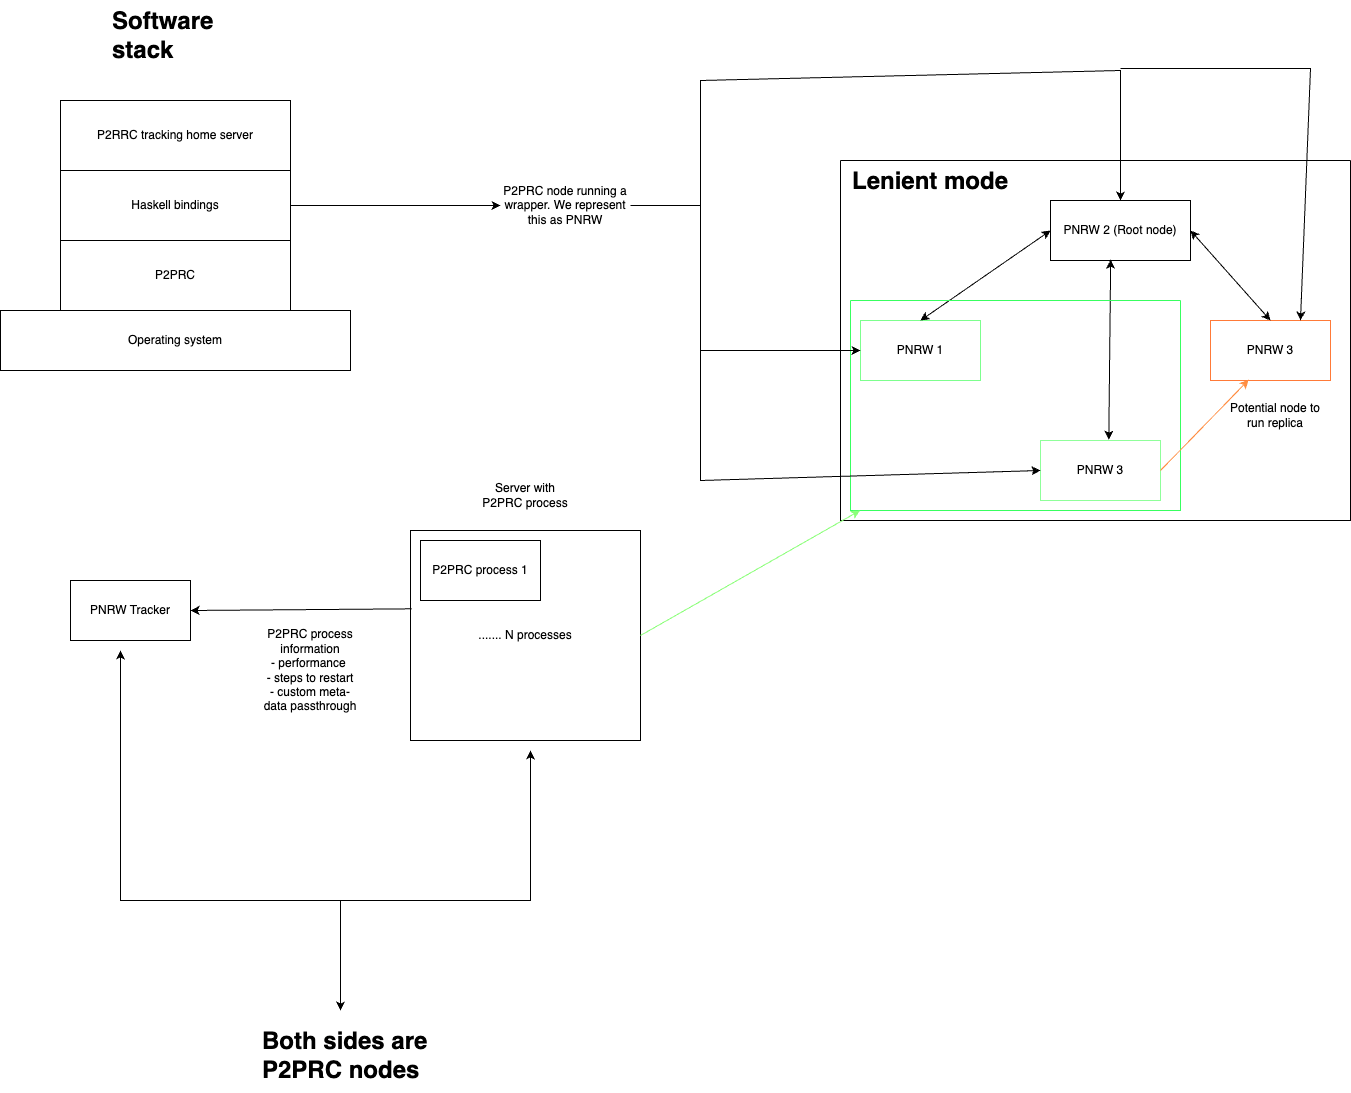
\includegraphics[width=.9\linewidth]{./P2PRC-Tracking-home-server.png}
\end{center}

\subsection{Plan}
\label{sec:org75ecafe}
Based on the \href{https://github.com/Akilan1999/p2p-rendering-computation/tree/master/haskell}{Haskell bindings} to build an extended library (There are still changes needed
in the Haskell bindings before the add-on can be built). 

\subsubsection{Handle more cases than machine name}
\label{sec:org7ed06ae}
The current haskell library seems to only support 1 type Machine name which is parseable from
the config file. We would need to handle conditions such as handling types such as \href{https://github.com/Akilan1999/p2p-rendering-computation/blob/67165d4bf63d82794a1a264edf843295b727c226/config/config.go\#L39}{Baremetal} and \href{https://github.com/Akilan1999/p2p-rendering-computation/blob/67165d4bf63d82794a1a264edf843295b727c226/config/config.go\#L40}{UnsafeMode}.
On this proposed library they would both be set to true. 
\begin{verbatim}
instance FromJSON P2prcConfig where
parseJSON (Object o) = do

  machineName <- o .: "MachineName"

  pure
    $ MkP2prConfig
      { machineName=machineName
      }

parseJSON _ = mzero
\end{verbatim}

\subsubsection{Representation of a process}
\label{sec:orgd88a8e7}
To design a data structure that can represent current set of properties:
\begin{enumerate}
\item IP address (string)
\item Port no (int)
\item Task name (string)
\item Task id (int)
\item Encoded deployment script (multi-line string)
\item Command to run deployment script (multi line string)
\item Command to kill deployment script (multi line string)
\item Status (boolean)
\item Domain name (string)
\end{enumerate}

\subsubsection{Representation of a node:}
\label{sec:orga084f25}
Follows the implemented Haskell data structure from the bindings:
\begin{verbatim}
instance FromJSON ServerInfo where
parseJSON = withObject "ServerInfo" $
  \ o -> do

    name        <- o .: "Name"
    ip4str      <- o .: "IPV4"
    ip6str      <- o .: "IPV6"
    latency     <- o .: "Latency"
    download    <- o .: "Download"
    upload      <- o .: "Upload"
    serverPort  <- o .: "ServerPort"
    bmSshPort   <- o .: "BareMetalSSHPort"
    nat         <- o .: "NAT"
    mEscImpl    <- o .: "EscapeImplementation"
    custInfo    <- o .: "CustomInformation"
\end{verbatim}

\subsubsection{Function expected to be built:}
\label{sec:org4644889}
The following refers to the functions we would be building for our abstraction:
\begin{enumerate}
\item SpinProcess(<P2PRC process type>,<Node Type>)
\item KillProcess(<P2PRC process type>)
\item ProcessInformation(<process id> or <domain name>) returns <P2PRC process type>
\item ListProcess() return <P2PRC process type>
\end{enumerate}

\subsection{Terms}
\label{sec:orgd859ef0}
P2PRC process: A p2prc process refers to potentially an instance (i.e web-server or any task). This process
stores information such as:
\begin{itemize}
\item Memory usage.
\item Instructions to re-produce that task etc\ldots{}
\end{itemize}

Root node: Refers to a node running P2PRC with a public IPV4 address to relay traffic through for nodes
behind NAT and can potentially even act a proxy for nodes(Used for domain name mapping) in the P2P network.  
\end{document}